












































\section{Results}

\subsection{Steady-state Approximation of Effective Viscosity}
\label{sec:eff_vic}
We begin with a calculation of a strain rate estimate of the effective viscosity for a network described by our model in the limit of highly rigid filaments.  We carry this out by assuming we have applied a constant stress along a transect of the network.  With moderate stresses, we assume the network reaches a steady state affine creep. In this situation, we would find that the stress in the network exactly balances the sum of the drag-like forces from cross-link slip.  So for any transect of length D, we have a force balance equation.

\begin{equation}
\mathbf{\sigma} = \frac{1}{D}\sum_{filaments}\: \sum_{crosslinks}\xi \cdot (\mathbf{v_i(x)}-\mathbf{v_j(x)})
\end{equation}

where $\mathbf{v_i(x)}-\mathbf{v_j(x)}$ is the difference between the velocity of a filament, $i$, and the velocity of the filament, $j$, to which it is attached at the cross-link location, $\mathbf{x}$. We can convert the sum over cross-links to an integral over the length using the average density of cross-links, $1/l_c$ and invoking the assumption of (linear order) affine strain rate, $\mathbf{v_i(x)}-\mathbf{v_j(x)}=\dot \gamma x$. This results in

\begin{multline}
\mathbf{\sigma} =  \frac{1}{D}\sum_{filaments}\:  \int_0^L \xi \cdot  \: (\mathbf{v_i(s)}-\mathbf{v_j(s)}) \:\frac{ds \cos \theta }{l_c} \\
 = \sum_{filaments}\:  \frac{\xi \dot \gamma L}{l_c} \cos \theta \cdot (x_l + \frac{L}{2} \cos \theta)
\end{multline}

Here we have introduced the variables $x_l$, and $\theta$ to describe the leftmost endpoint and the angular orientation of a given filament respectively.  Next, to perform the sum over all filaments we convert this to an integral over all orientations and endpoints that intersect our line of stress. We assume for simplicity that filament stretch and filament alignment are negligible in this low strain approximation.  Therefore, the max distance for the leftmost endpoint is the length of a filament, L, and the maximum angle as a function of endpoint is $\arccos(x_l/L)$.  The linear density of endpoints is the constant $D/l_cL$ so our integrals can be rewritten as this density over $x_l$ and $\theta$ between our maximum and minimum allowed bounds.

\begin{equation}
\mathbf{\sigma} =  \frac{1}{D} \int_0^L dx_l \int_{-\arccos (\frac{x_l}{L})}^{\arccos (\frac{x_l}{L})}\frac{d\theta}{\pi} \frac{\xi \dot \gamma L}{l_c} \cdot \frac{D}{Ll_c}\cdot (x_l \cos \theta + \frac{L}{2} cos^2\theta)
\end{equation}

Carrying out the integrals and correcting for dangling filament ends leaves us with a relation between stress and strain rate.

\begin{equation}
\mathbf{\sigma} = \frac{(L-2l_c)^2 \xi}{4\pi l_c^2} \dot \gamma 
\end{equation}

We recognize the constant of proportionality between stress and strain rate as a viscosity.  Therefore, our approximation for the effective viscosity, $\eta_{eff}$, at steady state creep in this low strain limit is

\begin{equation}
\label{lin_eqn}
\eta_{eff} = \frac{(L-2l_c)^2 \xi}{4\pi l_c^2} .
\end{equation}

As illustrated in Figure \ref{fig:effvic}, under moderate strains ($\gamma<0.2$), our  simulations show that in the high density limit, our theoretical approximation from Eqn \ref{lin_eqn} is highly accurate at explaining the network behavior.  Aside from a geometrical factor, our approximation is valid for both shear and extensional stresses applied to the network.

As the density of the network approaches the breakdown limit, the effective viscosity diverges from our expected value.  At the low connectivities, our expected viscosity goes to 0, but the medium viscosity begins to take over as we cross the percolation threshold at $L/l_c \sim 6$.  
\begin{figure}[h!]
\centering
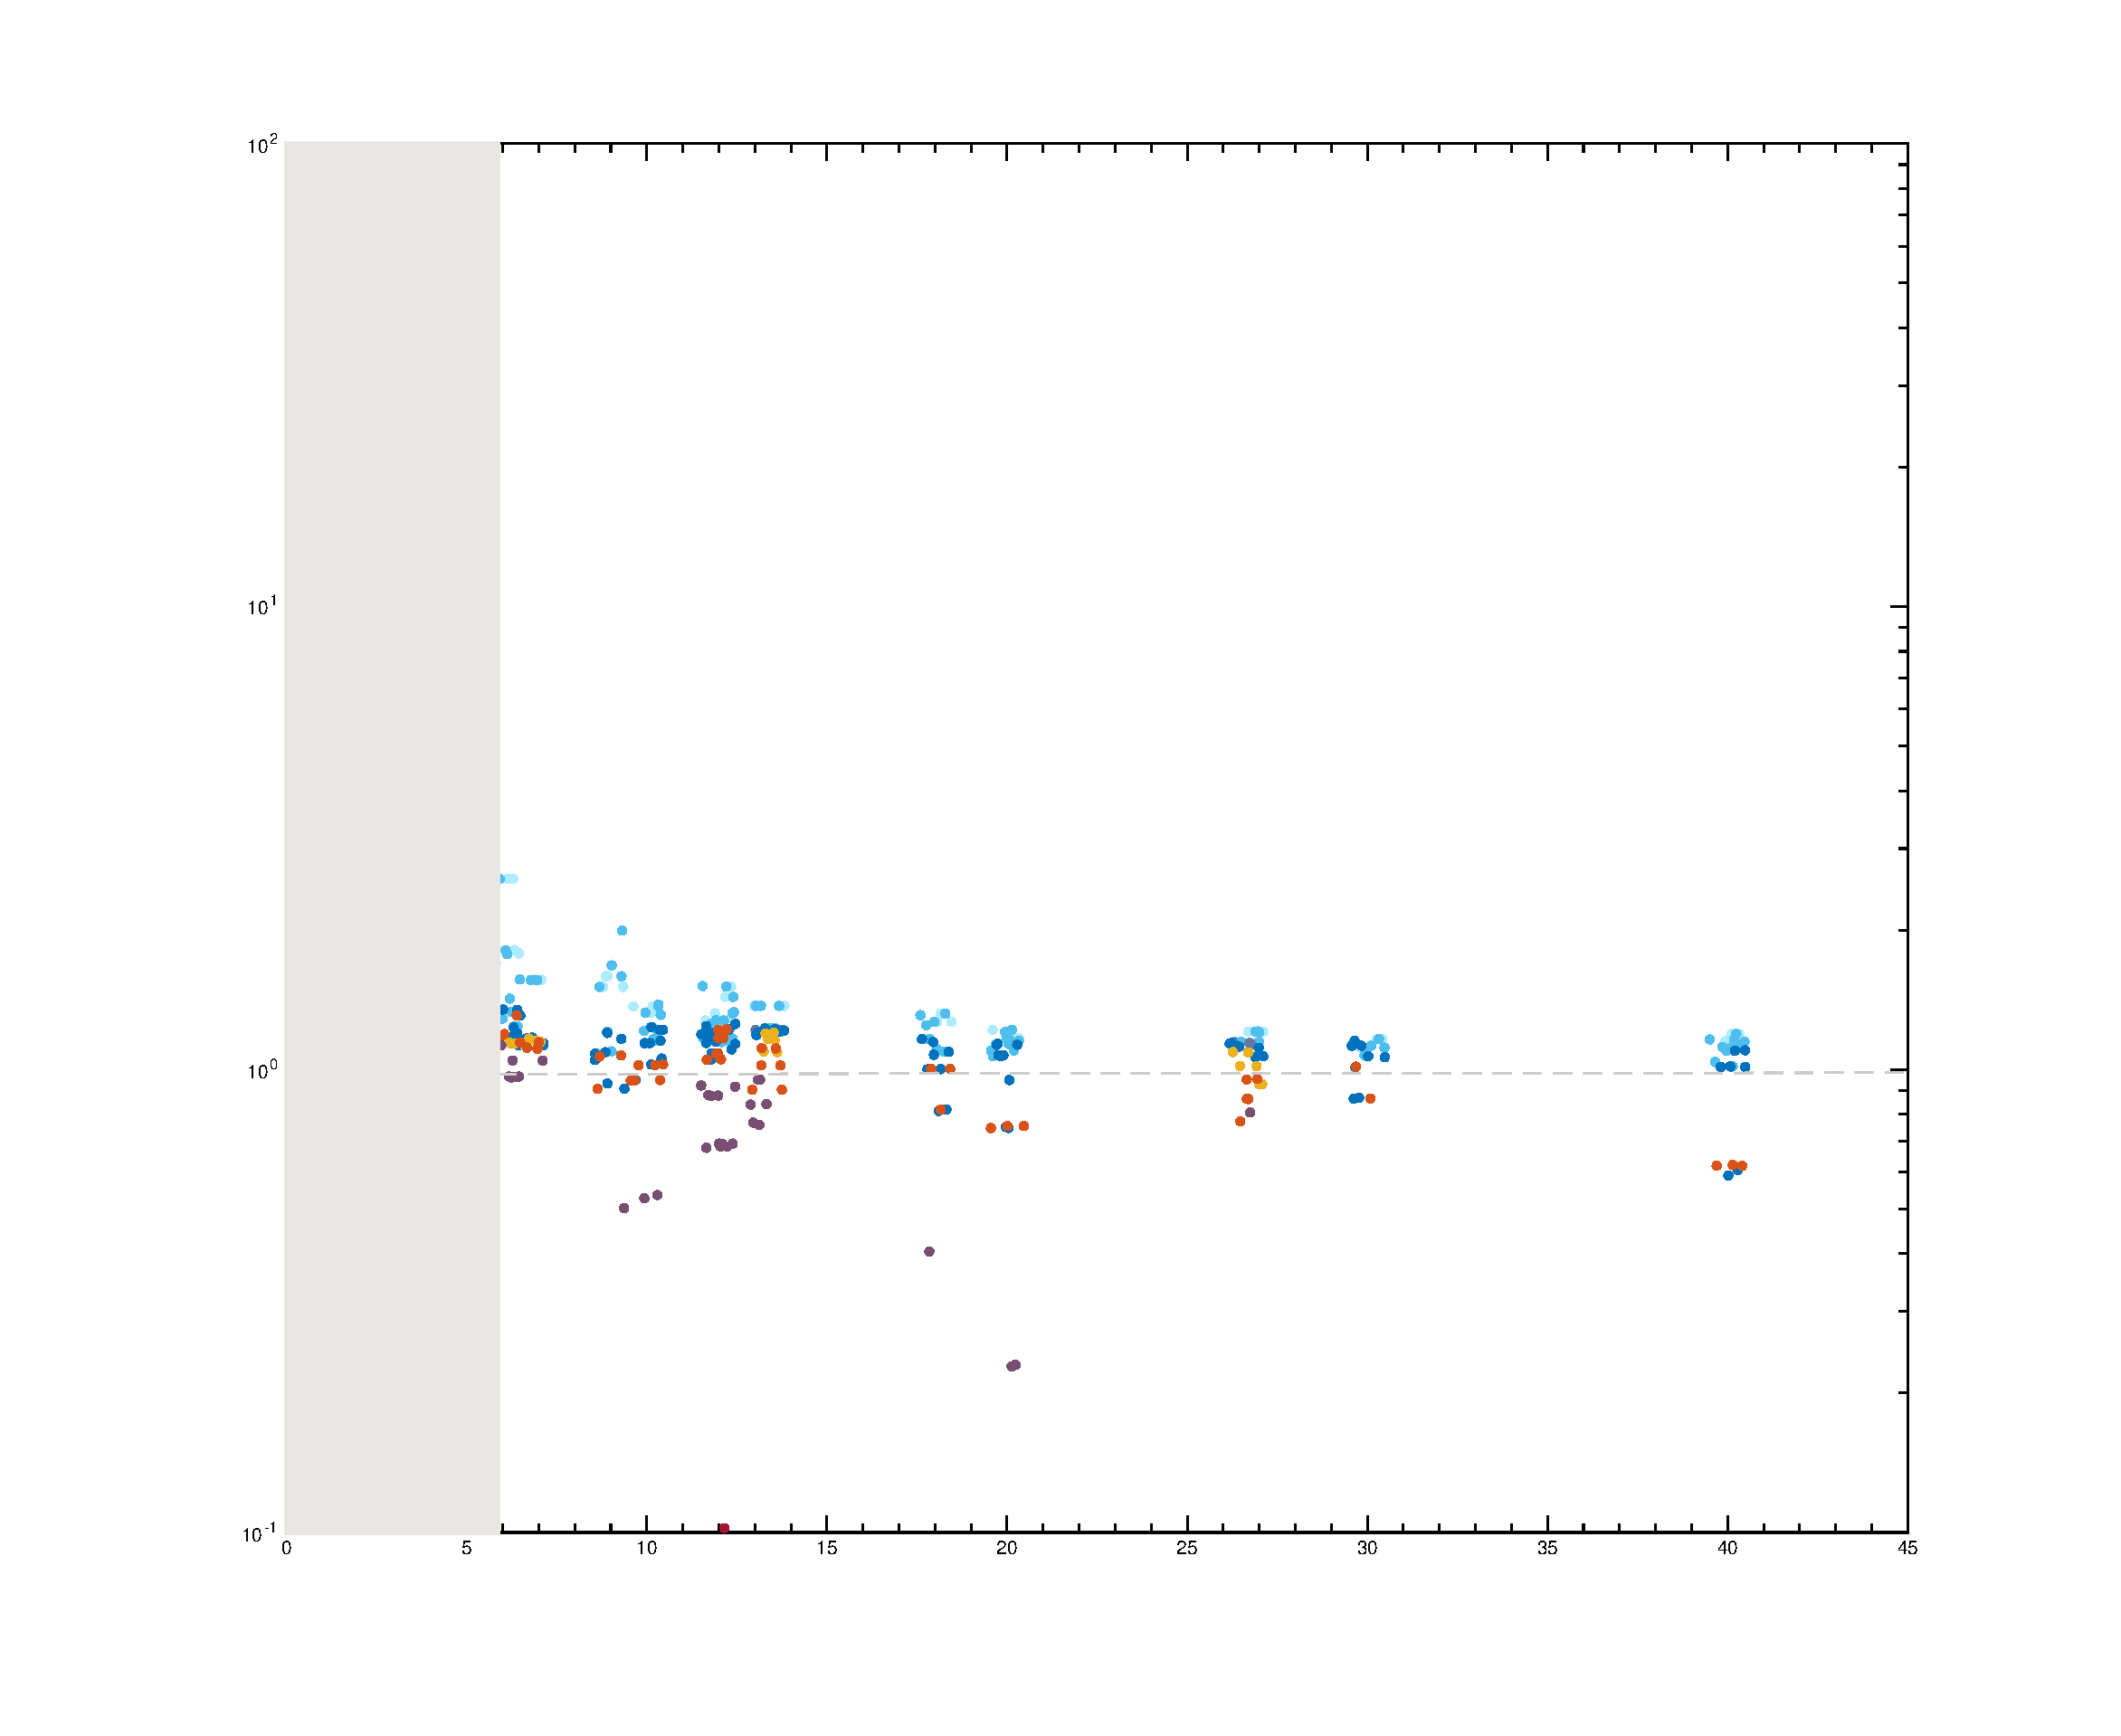
\includegraphics[width=\hsize]{slippage/eff_vic_master}
\caption{\label{fig:effvic}Ratio of effective viscosity measured by shear simulation to predicted effective viscosity as a function of connectivity, $L/l_c$. Inset: Same measurement for extensional simulations }
\end{figure}

In addition to changing the architecture and effective drag coefficient, we also validated the generality of our approximation by varying simulation size, medium viscosity, filament stiffness, and applied stress.  We were able to find a slight trend that depended on filament stiffness as indicated in the difference between blue and red data points in Figure \ref{fig:effvic}.  The deviation from our approximation and variability in results manifested itself more strongly when filaments were highly compliant.  To investigate this effect further, we next performed a more detailed analysis of the creep response while varying filament compliances.



\subsection{Effects of Filament Compliance}
\label{sec:compliant}


The effect of filament compliance on cross-linked networks under strain is a subject of active research at the moment [Sayantan].  Therefore, we wished to use our computational approach to extend our understanding of filament networks in the regime of non-negligible filament compliance.  

In irreversibly cross-linked polymer networks, filament compliance is known to give rise to elastic deformation of the network as described in\cite{theo_hlm,theo_hlm2}.    

During the initial affine deformation immediately after the application of an external stress, we see a rapid stretch of filaments, $\langle \delta L/L\rangle_0$, in response to the affine purely mechanical strain, $\gamma_{xy}$, which closely follows $\langle \delta L/L\rangle_0 = \gamma_{xy}sin(\theta)cos(\theta)$. As shown in Figure \ref{fig:glass_relax}, during the first phase in our simulations, the total network strain (solid) is described almost entirely by the strain of the filaments (dotted).  

However, in the presence of cross-link slip, the filaments are not permanently constrained to remain at $\langle \delta L/L\rangle_0$.  Interestingly, although the mean filament strain stays approximately constant, the distribution of individual filament strains broadens around the affine approximation as shown in the inset of Figure \ref{fig:glass_relax}.  

During the period where crosslink slip allows changes in the filament length distribution, we also find a long-lived intermediate relaxation phase that deviates from both the initial purely elastic relaxation and the later purely viscous behavior of section \ref{sec:eff_vic}.  In Panel B of Figure \ref{fig:glass_relax}, we show that the standard deviation of the filament stretch distribution continues to increase throughout the period that the strain rate is non constant.   

Approximating this broadening as a normally distributed variation in filament stretched length throughout the network ($\mathcal{N}$) with a time varying standard deviation, $\sigma(t)$, we have $\delta L/L = \langle \delta L/L\rangle_0 + \sigma(t)\cdot\mathcal{N}$. 
 This has an effect on the total mechanical energy stored in the network ${\cal H} \sim  \langle\delta L/L\rangle^2 = \langle\delta L/L\rangle_0^2 +\sigma(t)^2 $.   Therefore, the network will deform further while some strain energy is being stored in the further stretching filaments.  



\begin{figure}[h!]
\centering
\includegraphics[width=\hsize]{slippage/glass_relax_illustrate}
\caption{\label{fig:glass_relax} Network and filament strain for different filament drag coefficient parameters.  (top) Plot of total strain normalized by the final mean filament strain, $\delta L/L$.  Dashed lines show the amount of strain from affine mechanical stretching.   (bottom) Standard deviation of filament extension for the networks in A. Note that the creep compliance in A becomes constant (slope 1) only after the spread in filament extension in B stops increasing.  Colors indicate unique experimental conditions. }
\end{figure}



Eventually the contribution from slow filament stretching will become negligible compared to that from pure cross-link slip on rigid rods.  This occurs on a timescale similar to that of cross-link slip and causes the effective viscosity to decay back toward the rigid limit.  This gives rise to a less-than-linear creep response during times after the initial elastic relaxation but before full filament relaxation from cross-link slip.   As shown in Figure \ref{fig:strain_coll}, the transition begins to take place as network strain reaches 10 to 100 times the strain from pure mechanical stretching, $\gamma_0 = \delta L / L$, and this property is independent of the magnitude of the rate of strain.  

\begin{figure}[h!]
\centering
\includegraphics[width=\hsize]{slippage/collapse}
\caption{\label{fig:strain_coll} Sublinear network strain ends as change in filament strain decays. (top) Change in standard deviation of filament strain, $\sigma$, as a function of strain relative to pure mechanical strain. (bottom)   Dependence of strain rate exponent as a function of strain relative to pure mechanical strain, $\gamma_0$.  Colors indicate unique experimental conditions. }
\end{figure}




















\subsection{Alignment at High Strain and Network Tearing}

Once the network is able to accumulate a large strain, the assumption of nearly uniform distributions of filament orientations begins to break down.

At this point the filament orientations become unevenly distributed $\langle \delta L / L \rangle \neq \gamma_{xy}sin(\theta)cos(\theta)$, with a larger number of filaments aligning in the direction of extension rather than compression.  Filament alignment, conceptually, causes the formation of subdomains that no longer span the space of the network. To the authors' knowledge an exact derivation of the dependence of network connectedness on filament alignment has not been carried out, but Monte Carlo simulations have been used to show that alignment does indeed lead to lower connectedness\cite{model_percolationanisotropy}.

\begin{figure}[h!]
\centering
\includegraphics[width=\hsize]{slippage/tearer}
\caption{\label{fig:tearer} Creep response of a network transitioning to phase D. (top)  Strain curves for a network undergoing large scale deformation.  Inset shows strain exponent as a function of strain (exponent passes 1).  (bottom)  Traces for the variance in filament orientation and number of cross links.  Vertical dashed line shows the point where the strain exponent becomes greater than one.}
\end{figure}

We find that over time, the orientational distribution of the filaments begins to peak around 45 degrees as the large strain induces alignment.  In Figure \ref{fig:tearer}, we see that as the angular standard deviation falls, this reorientation eventually leads to fewer bonds bridging the network perpendicular to the line of strain.  As this connectivity begins to noticeably decrease, the observed effective viscosity decreases as well, giving rise to greater than linear creep.  From the inset of Figure \ref{fig:tearer} we can also see that the onset of phase D occurred before the network had completely reached phase C, leading to a rapid transition between sub-linear and super-linear creep.  Finally, it should be noted that the end of this simulation resulted in the network tearing apart.  



\subsection{Phase Diagram of Dominant Behavior}
In Figure \ref{fig:shear_modes}, we illustrate the four stereotyped phases of the general mechanical behavior that we observed in our networks.  A deforming network typically undergoes a rapid filament stretching, a slower relaxation of elastic constraints, a phase of purely viscous cross-link slippage, and an eventual alignment and breakdown of network connectivity.

\begin{figure}[h!]
\centering
\includegraphics[width=\hsize]{slippage/shear_modes_b}
\caption{ \label{fig:shear_modes} Schematic of the general creep response of compliant filament networks illustrating the 4 phases of deformation: A) rapid mechanical response, B) combination of slow filament stretching and cross-link slip, C) cross-link slip dominated (line indicates slope of one), D) network tearing from filament alignment. Note that the portion of the curve in section D is only a hypothetical continuation of the actual data.  }
\end{figure}


Finally, to explore the transitions between the various phases, we measured the creep response for a computationally tractable network ($L/l_c = 25$), as we varied the filament extensional modulus, $\mu$, and the cross-link friction coefficient, $\xi$.  In Figure \ref{fig:phase_diag}, we classified parameter sets based on their strain exponent.  We can see the trends for the transitions between phases A, B, and C.  The line for the transition to D is still speculative at this time.  

\begin{figure}[h!]
\centering
\includegraphics[width=\hsize]{slippage/phase_diag}
\caption{\label{fig:phase_diag} phase diagram of creep response for different filament extension, $\mu$ and cross-link friction, $\xi$.  Yellow, green, and purple dots correspond to creep measurements $\gamma \sim t^\alpha$ with $\alpha<0.92$, $0.92<\alpha<0.98$, or $\alpha>0.98$ respectively.  Blue dots represent creep measurements where $\gamma_{total} < 2\gamma_{mechanical}$}
\end{figure}

\subsection{Frequency dependent modulus}
This section will include a figure on the frequency dependent modulus once I get those.

\begin{figure}[h!]
\centering
\includegraphics[width=\hsize]{slippage/frequency_dep}
\caption{\label{fig:freq} Frequency dependent moduli for networks.}
\end{figure}



\subsection{Strain Memory}
Finally, we found an interesting behavior when we introduced non-linear extensional stiffness into our filaments.  When the network is allowed to relax to it's unstrained state, there is generally a time comparable to the period of strain storage over which the energy in the network is relaxed away.  

We observed deviations from this behavior by applying stepwise stress pulses to simulated networks, and observing whether the network behaves identically upon reversal of the applied stress direction.  If the network has no strain memory then each reversal will result in an identically shaped creep curve.  However, when we include nonlinear filament extension in our model, we find that the mechanical strain can be stored for longer periods of time than it took to entrain the network.

This behavior mimics recent experiments in filamin cross-linked networks.  Filamin provides a high level of compliance to a network ($\gamma_0>0.5$) without substantial cross-link unbinding.  This allows large scale rearrangements to take place without driving very much cross-link slip, similar to the conditions in section \ref{sec:compliant}.  However, if we force individual filaments to undergo a strongly nonlinear stiffening at strains above 5\%, we find an interesting long term "strain storage."

\begin{figure}[h!]
\centering
\includegraphics[width=\hsize]{slippage/strain_mem_weak}
\caption{\label{fig:strain_mem_weak} Creep curves in the presence of reversing applied stress for (a) nonlinear extension or (b) linear extension.  Note that for linear filaments the induced strain returns to approximately 0 after a complete cycle, while in the nonlinear case the cycle is not completely reversible.}
\end{figure}

Figure \ref{fig:strain_mem_weak} shows that the strain storage occurs, but I will need time for further study to build the full analytical picture of where when and why this happens in my model.













\section{Summary and Conclusions}
We have proposed a simplified effective friction model for understanding 2D cross-linked networks. Our model extends previous Mikado and lattice models to include effects of cross-link relaxation. We expect that our model can confer insights into mechanisms of network stress relaxation in quasi-2D networks such as those found in \textit{in vitro} actin monolayer experiments\cite{rheo_2D1} as well as in eukaryotic actomyosin cortices\cite{cellmech_flows}.   

Our model is the first to address the plausible dependence of network effective viscosity on network structural properties.  This led to a derivation of an estimate for the long timescale creep rate of networks under constant stress.  Although this derivation neglects possible frequency dependence at short timescales, this finding offers a potential framework for addressing the dependence of network deformation rate on filament concentration and length.

Additionally, our simulations suggest that, in the presence of constant shear stress, cross-link friction will also produce a long-lived phase of sublinear creep as filaments relax from their affine stretched position. While this phase may transiently resemble more explicit 3D models such as \cite{theo_crosslinkslip1}, it is clear that our model differs by predicting that network will achieve a constant effective viscosity more rapidly.  In particular, we predict that this relaxation will occur at a rate similar to that of rate of cross-link slip derived strain and will therefore be negligible after the network has slipped by roughly ten times the magnitude of the purely affine mechanical deformation.  

In building our model we have neglected any other sources of potential mechanical relaxation in order to simplify out analysis. In the future, we hope to extend our model to include biochemically driven forms of relaxation such as filament turnover or regulated cross-link unbinding.

This model forms a basis for addressing 2D filament network deformation, and it proposes a simplified formulation of important qualitative properties. In this way we are able to address potentially general phases of network deformation and delineate what network properties may give rise to them.  This may provide an important starting point for addressing the general importance of network structure in more complex networks containing active elements. 






































\section{Network Tearing under Extensional Stress}


\subsection{Extensional Thinning and Network Tearing}

For moderate extensional stresses, the rigid filament approximation of the effective viscosity simply picks up a different geometrical factor out front.  

However, at higher stress and in the presence of different things happen.

\begin{equation}
\frac{\partial l_c}{dt}=l_c\dot \gamma =\frac{l_c \sigma}{\eta}\sim l_c^3\frac{ \sigma}{L^2 \xi}
\end{equation}

We can see that the rate of network thinning accelerates as we would expect.  When the network reaches some minimum connectivity we assume that it stops behaving as a continuum material and the network tears irreversibly.  

\begin{equation}
\tau_{break} = \frac{\eta_{eff}}{2\sigma}\cdot\left ( 1 -\frac{l_c^2}{l_{break}^2} \right )
\end{equation}

This provides us with an estimate of the timescale of catastrophic breakdown for a network with a given initial architecture and molecular drag.


\subsection{Tearing Events During Extensional Strain}

This behavior is caused primarily by the low density network undergoing tearing events that interrupt global connectedness.  




\section{Deriving Molecular Drag Coefficients}
\label{app:drag}
Thus far, the idea of a molecular drag coefficient was taken as a phenomenological, measured parameter for a given experimental setup.  While this is a sufficient pragmatic justification, it's useful to try to motivate the quantitative value of this drag coefficient by connecting it to the underlying cross-link properties of binding affinity, concentration, and extensibility.

To do this we'll imagine the simplified case of two cross linkers sliding past each other in one dimension.  In this case, assume that we have an equilibrium number of bound cross-linkers, $n_B$, each of which is displaced from its equilibrium length by some distance $x$.  Each cross linker unbinds with rate $k_{off}$ and rebinds at it's relaxed position ($x=0$) with rate $k_{on}$.  At the same time, all the cross linkers are being pulled from their relaxed position at a rate, $v$, which is simply the rate at which the filaments are sliding past each other.  

We can write the differential equation for the change in the density of cross-links, $\rho$, at displacement $x$ as they are pulled upon, bind, and unbind.

\begin{equation}
\frac{\partial \rho}{\partial t} = -k_{off}\rho(x) - v\frac{\partial \rho}{\partial x} + k_{on}\delta(x)
\end{equation}

Recognizing that $\int \rho(x)=n_B$ implies $k_{on}=k_{off}n_B$, we can find the steady state solution

\begin{equation}
\rho(x) = \frac{n_b k_{off}}{v}\cdot exp\left ( -\frac{k_{off}}{v}x \right )
\end{equation}

If each cross-link has a spring constant $\mu_c$, then we can equate the force on all cross-links to the applied force that is sliding the filaments past each other.  Realistically, the spring constant and binding affinity would be functions of the cross-link stretch, but here we are taking them as approximately constant.  

\begin{equation}
\int_{0}^{\infty}\rho(x)\mu_cx dx = v \frac{\mu_c n_B}{k_{off}}= F_{app}
\end{equation}a

Therefore, the term next to v, (i.e. $\tfrac{\mu_c n_B}{k_{off}}$) would be equal to our molecular drag coefficient, $\xi$.  Assuming approximately 1 cross link per filament overlap, and using parameter estimates culled from Ferrer et al., we build the following table of estimates for $\xi$.

\begin{table}[h]
\begin{tabular}{| l | c | c |}
\hline
\textbf{cross-linker type} & $\alpha$-actinin & filamin-A  \\ \cline{1-1}
\textbf{dissociation constant ($s^{-1}$)} & 0.4 & 0.6 \\ \cline{1-1}
\textbf{spring constant ($nN / \mu m$)} & 455 & 820 \\ \cline{1-1}
\textbf{drag coefficient, $\xi$ ($\tfrac{nN \cdot s}{\mu m}$)} & 182 & 492 \\ 
\hline
\end{tabular}
\end{table}



This molecular description assumed both a constant off-rate and linear force extension of cross-links.  In the event that binding kinetics are regulated by the state of extension, we would expect (based on Rf) to find a region that exhibits a stick-slip behavior instead of the smooth.  Depending on the nature of any coupling between cross-links local stick-slip could either give rise to a global stick-slip behavior or a heterogenous mixture of stuck and sliding cross-links.  It would be interesting to explore this topic further in the future, but in the present analysis, we choose to ignore complications from these nonlinear effects.


